% -*- root: ./report.tex -*-
\chapter{Methods}\label{chap:methods}

\section{Physical picture}\label{sec:physical_picture}
	\comment{We consider a two-dimensional system with zigzag.}
	We consider a Josephson junction (JJ)(Fig.~\ref{fig:setup}) consisting of a two dimensional strip of semiconductor, with superconductors on both sides.
	We modulate the shape of the normal region, which can be either zigzag as depicted, or a more smooth sinusoidal like shape.
	Similar to the conventional straight system \cite{pientka_topological_2017}, a magnetic field $B_x$ is applied, along the x-axis.
	We model the system with a BdG Hamiltonian, Eqs.~\eqref{eq:hamiltonian_n}-~\eqref{eq:hamiltonian_s}  ; the normal part has a linear Rashba spin-orbit coupling term characterized by the spin-orbit strength $\alpha$ , and a Zeeman energy $E_z= mu_B g B_x$.
	The superconductor has a superconducting coupling term $\Delta$ with a superconducting phase $\pm\phi/2$ (the phase difference between the superconductors is $\phi$).
	Both parts have a kinetic term and chemical potential $\mu$ (counted from the bottom spin-orbit band). 
	For the zigzag geometry, we first consider a sawtooth like pattern where $z_y$ is the amplitude, $z_x$ is the period, and $W$ the width of the junction.

	\begin{figure}[!htb]
	\centering
	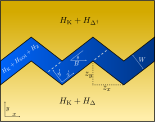
\includegraphics[width=0.5\columnwidth]{images/zigzag.pdf}
	\caption{Figure of a zigzag system.
	$z_x$, $z_y$ and $W$ describe the geometry of the zigzag junction.
	$H_\text{K}$ describes the kinetic part of the Hamiltonian, $H_\text{SOI}$ is the spin-orbit term, $H_\text{Z}$ is the Zeeman coupling, and $H_\Delta$ represents the superconducting term.
	The magnetic field (B) points along the x-axis.
	\label{fig:setup}}
	\end{figure}

	\begin{align}
	    H_\text{N} &= \left(\frac{\hbar^2\left(\kx^2 + \ky^2\right)}{2\meff} - \mu + \frac{\meff \alpha^2}{2 \hbar^2} \right) \left( \sigi \otimes \tauz \right)+
	        E_\text{z} \left(\sigx \otimes \tauz \right) +
	        \alpha \left( \ky \sigx - \kx \sigma_y \right) \otimes \tauz \label{eq:hamiltonian_n} \\
	    H_\text{SC} &= \left(\frac{\hbar^2\left(\kx^2 + \ky^2\right)}{2\meff} - \mu \right) \left(\sigi \otimes \tauz \right) +
	        \Delta \left(\sigi \otimes \tau_{\pm \phi /2}\right)
	\label{eq:hamiltonian_s}
	\end{align}
	where,
	\begin{equation}
	    \tau_{\pm \phi /2} = \cos\left( \pm \phi /2 \right) \taux + \sin\left( \pm \phi /2 \right) \tauy \nonumber
	\end{equation}

\subsection{Symmetry class of system}
	\comment{The symmetry class of the system is D.}
	The non-zigzag system is in the symmetry class BDI \cite{pientka_topological_2017}, unless the additional symmetries are broken due to for example a difference in superconducting gap magnitude between the two superconductors.
	Using the software package Qsymm\cite{varjas_qsymm_2018}, we find that the symmetry class of our system to be D, because we break this chiral/time-reversal symmetry resulting from the mirror symmetric junction.


\section{Tight binding simulation}

	\comment{We use kwant to make systems and extract the eigenstates}
	We use a tight-binding model, implemented using Kwant, to simulate various properties of the system.
	The model consists of a two-dimensional square lattice of sites.
	Each site has two orbitals: spin and electron-hole.
	There are four different types of sites (and thus four different Hamiltonians): the top superconductor, the bottom superconductor, the normal region, and a normal region with an optional potential offset, acting as a barrier to simulate an imperfect NS interface.
	A schematic of such kwant systems is depicted in Fig.~\ref{fig:kwant_system}.

	\comment{The model hamiltonian is converted into the tight binding form by substitution}
	In order to turn the set of Hamiltonians, Eqs.\eqref{eq:hamiltonian_n} and \eqref{eq:hamiltonian_s} into a tight binding model, we write the equations into differential form by substituting $k_\alpha \rightarrow - i \partial_\sigma$, $\sigma \in \left\{ x, y \right\}$, and thereafter discretize on a rectangular grid.
	In practice, this is implemented using the Kwant discretizer module.


	\begin{figure}[!htb]
	\centering
	\includegraphics[width=0.95\columnwidth]{figures/kwant_system}
	\caption{Figure of different examples of simulated systems in Kwant.
	Lattice spacing is made bigger to make the discretization visible.
	The two golden regions are both superconducting, but differ in phase.
	The blue and black regions form the semiconductor, but the black region has an optional potential offset to model an imperfect interface, increasing the amount of normal reflection.}
	\label{fig:kwant_system}
	\end{figure}


	\comment{We extract the gap by either taking the lowest energy state for an infinite system, or the difference between the lowest two eigenstates.}
	After the system is specified, we can extract the total Hamiltonian of the system, allowing analysis of the eigenstates.
	For example, calculating the bandstructure of a system is performed by taking a translationally invariant system and calculating the eigenvalues for different momenta.
	The system is made translationally invariant, in for example the $x$ direction, by connecting the sites on the left border with those on the right border with a $\kx$ dependent hopping.

	\comment{We propose a method to verify that elimination of long trajectories is responsible for the increased topological gap in a zigzag system.}

\section{Quasiclassical estimation of the topological gap}
	\comment{To compute the effect of cutoff consider a single segment of the zigzag and obtain the spectrum analytically (this allows to use translation invariance).}
	To establish that the elimination of long trajectories is indeed the driving mechanism behind the improvement of the gap, we use an analytical model in an effort to isolate the gap-trajectory dependence.
	We estimate the gap of the zigzag system by the minimum energy occuring in the Andreev spectrum of a single (diagonal) segment of zigzag (see Fig.~\ref{fig:zigzag_methods}).
	We define the spectrum of a single zigzag segment by identifying it with the spectrum of an infinite ribbon SNS junction with tilted-magnetic field.
	The finite length of the segment is modeled by not including momenta corresponding to long trajectories when taking the minimum over the spectrum.

	\comment{The spectrum is derived using a scattering matrix, and we consider multiple ways to eliminate long trajectory momenta.}
	Estimating the gap is a two-step process: first, derivation of the Andreev spectrum, and second, taking the absolute minimum of that spectrum over the set of momenta allowed by the specific geometry.
	An analytic expression for the spectrum is derived using scattering matrix formalism and the Andreev bound state condition\cite{beenakker1991universal, sticlet_robustness_2017}.
	For the second step, the difficulty lies with identifying the set of allowed momenta in a particular geometry.


	\subsection{Analytical estimate of Andreev spectrum for a straight junction}
		
		We derive the spectrum by calculating the scattering matrix for the normal region and applying the Andreev bound state condition for the short junction limit\cite{beenakker_universal_1991,sticlet_robustness_2017}.. 
		The short junction limit is valid for $W<\xi$, where $\xi$ is the superconducting coherence length.
		For deriviation of the scattering matrix, we neglect SOI in the transverse direction, which is valid for $W<l_\text{so}$.

		\subsubsection{Derivation of the scattering matrix}

			\begin{figure}[!htb]
			\centering
			\includegraphics[width=0.75\columnwidth]{images/scattering}
			\caption{Basis for scattering matrix. 
			The `S' region corresponds to the superconductor Hamiltonian without the superconducting term, Eq.~\eqref{eq:ham_smat_superconducting}, `N' to the normal region, Eq.~\eqref{eq:ham_smat_normal}. 
			The coefficients (corresponding to the scattering problem outlined in Eqs.~\ref{eq:scattering_matrix_problem} and \ref{eq:scattering_equations}) represent the amplitude of the modes present in the system, at a particular energy.
			The different color arrows correspond to the two different spinors in each region.
			For example, $a_{1,L}$ is the amplitude of the rightmoving incoming mode, $\vec{\psi}_1 \exp\left(i k_{1,L} x\right)$}
			\label{fig:scattering}
			\end{figure}
			
			\begin{align}
			H_\text{N} &= \left[ \frac{\hbar^2}{2 \meff} \left(\kx^2 + \ky^2\right) -\mu_n\right]\sigi +
						 \alpha \kx \sigy +
						 E_z \left[ \cos(\theta) \sigx + \sin(\theta) \sigy \right]
			\label{eq:ham_smat_normal} \\
			H_\text{S} &= \left[\frac{\hbar^2}{2 \meff} \left(\kx^2 + \ky^2\right) -\mu_s\right]\sigi
			\label{eq:ham_smat_superconducting}
			\end{align}
			
			We consider the scattering region as depicted in Fig. \ref{fig:scattering}.
			There are three regions in the system, one normal system (N), with Hamiltonian given by Eq.~\eqref{eq:ham_smat_normal}, and two superconducting regions (S), with Hamiltonian given by Eq.~\eqref{eq:ham_smat_superconducting}.
			Note that Eq.~\eqref{eq:ham_smat_superconducting} region does not include the superconducting term ($\Delta \tau_y$), because we implement Andreev reflection seperately (see Eq.~\eqref{eq:andreev_scat_mat})~\cite{beenakker_universal_1991}: this way we avoid doubling (electron and hole) the dimensionality of the problem.
			
			We set the energy of the system, and find the planar waves propogating in each region.
			Because the plane waves can go in two directions, and the additional degree of freedom introduced due to spin, each region has four propogating waves.
			The idea of the scattering matrix is to set the vector $\vec{a}$, containing the amplitudes of the planar waves coming in to the scattering region, and find the amplitudes of the modes exiting the scattering region.
			This is captured by a system of linear equations, displayed in Eq.~\eqref{eq:scattering_matrix_problem}.
			
			\begin{equation}
			\begin{bmatrix} 
			b_{1,L}\\
			b_{2,L}\\
			b_{1,R}\\
			b_{2,R}
			\end{bmatrix} 
			= S_\text{sns}(\epsilon) \cdot 
			\begin{bmatrix} 
			a_{1,L}\\
			a_{2,L}\\
			a_{1,R}\\
			a_{2,R}
			\end{bmatrix}
			\label{eq:scattering_matrix_problem}
			\end{equation}

			In order to find the coefficients of the matrix $S_\text{sns}(\epsilon)$, we take the wavefunction $u(x)$ and apply the boundary equations (continuity and flux conservation): specified in Eqs.~\eqref{eq:scattering_equations} through \eqref{eq:scattering_boundary_eqs}.
			Note that because we neglect spin-orbit coupling in the x-direction, the velocity operator $\hat{\mathbf{v}}$ can be simplified to the first derivative.
			Although omitted to keep the expression compact, the momenta $k_i, q$ and spinors $\vec{\Psi_{i, L/R}}$ are energy dependent.

			\begin{align}
				&u(x) = 
				\begin{cases}
				u_L(x) = a_{1,L} \vec{\Psi} _{s,1} \exp (i q y) + a_{2,L} \vec{\Psi} _{s,2} \exp (i q y) + b_{1,L} \vec{\Psi} _{s,1} \exp (-i q y) + b_{2,L} \vec{\Psi} _{s,2} \exp (-i q y)  & x \leq 0\\
				u_m(x) = d_{1,l} \vec{\Psi} _{n,1} \exp \left(-i k_1 y\right) + d_{1,r} \vec{\Psi} _{n,1} \exp \left(i k_1 y\right) + d_{2,l} \vec{\Psi} _{n,2} \exp \left(-i k_2 y\right) + d_{2,r} \vec{\Psi} _{n,2} \exp \left(i k_2 y\right)  & 0 \geq x \leq W\\
				u_R(x) = a_{1,R} \vec{\Psi} _{s,1} \exp (-i q y) + a_{2,R} \vec{\Psi} _{s,2} \exp (-i q y) + b_{1,R} \vec{\Psi} _{s,1} \exp (i q y) + b_{2,R} \vec{\Psi} _{s,2} \exp (i q y)  & W \geq x
				\end{cases}
				\label{eq:scattering_equations}
			\end{align}
				
			Where $a_{i, L/R}$ are the coefficients of the incoming modes, $b_{i, L/R}$ are those of the outgoing modes, and $d_{i, l/r}$ are the modes in the middle region: see Fig.\ref{fig:scattering}.
			The symbols $\vec{\Psi}_{n/s, i}$ and $k_i, q$ are respectively the spinors and corresponding momenta belonging to each region.
			Both are energy dependent.\\

			The boundary conditions are,
			\begin{align}
				& u(x) \text{ is continuous}\\
				&\hat{\mathbf{v}} u(x) \text{ is continuous, where $\hat{\mathbf{v}}$ is the velocity operator}\label{eq:scattering_boundary_eqs}
			\end{align}

			To solve the system analytically, we use the Short Junction limit: we set $E=0$ in Eq.~\eqref{eq:scattering_matrix_problem}.
			By applying the boundary conditions and solving the resulting linear system of equations, the resulting solution is given by Eqs.~\eqref{eq:smatrix} through ~\eqref{eq:momenta_short_junction}.
			\emph{Important note: In order to use the Andreev bound state condition, the scattering matrix must be in the correct basis. The relevant basis transformation has already been applied in Eqs. ~\eqref{eq:smatrix} through ~\eqref{eq:momenta_short_junction}}.\\
			
			Scattering matrix, in block matrix format:
			\begin{align}
			\label{eq:smatrix}
		    S &= \left(
		    \begin{array}{rr}
		    r_{ll}&t_{rl}\\
		    t_{lr}&r_{rr}\\
		    \end{array}
		    \right) =
		    \left(
		    \begin{array}{rr}
		    \beta_+ & e^{-i q W} \beta_-\\
		    e^{-i q W} \beta_- & e^{-2 i q W} \beta_+\\
		    \end{array}
		    \right)
		    \\
		    \beta_\pm &= \left(
		    \begin{array}{rr}
		    e^{i \nu_{\arg}}\left(\omega^\pm_1 - \omega^\pm_2\right) & (\omega^\pm _1 + \omega^\pm _2)\\
		    -(\omega^\pm _1 + \omega^\pm _2) & e^{-i \nu _{\arg }} \left(\omega^\pm _2 - \omega^\pm _1\right)\\
		    \end{array}
		    \right)\\
		    \omega^\pm_j &= \frac{1}{4} \left(\gamma _{j} \pm \delta _{j}\right)
			\end{align}

			Subexpressions:
			\begin{align}
			    \gamma_j &= \frac{q+i k_{j} \tan \left(\frac{W k_{j}}{2}\right)}{q-i k_{j} \tan \left(\frac{W k_{j}}{2}\right)} \\
			    \delta_j &= \frac{q-i k_{j} \cot \left(\frac{W k_{j}}{2}\right)}{q+i k_{j} \cot \left(\frac{W k_{j}}{2}\right)}\\
			    e^{i \nu_{\arg}} &= \frac{E_\text{z} e^{i \theta }-i \alpha  k_x}{\sqrt{E_\text{z}^2+\alpha  k_x \left(\alpha  k_x-2 E_\text{z} \sin (\theta )\right)}}
			\end{align}

			Momenta:
			\begin{align}
			    q &= \left[ \frac{2 m_\ast}{\hbar ^2}\mu_s - k_x^2 \right]^\frac{1}{2}\\
			    k_1 &= \left[ \frac{2 m_\ast}{\hbar^2} \left(\mu_n-\sqrt{E_z^2-2 \alpha  E_z \sin (\theta ) k_x+\alpha ^2 k_x^2}\right) - k_x^2 \right]^\frac{1}{2}\\
			    k_2 &= \left[ \frac{2 m_\ast}{\hbar^2} \left(\mu_n+\sqrt{E_z^2-2 \alpha  E_z \sin (\theta ) k_x+\alpha ^2 k_x^2}\right) - k_x^2 \right]^\frac{1}{2}
			\label{eq:momenta_short_junction}
			\end{align}

		\subsubsection{Resulting spectrum}
			In order to get the spectrum from the S-matrix [Eq.~\eqref{eq:smatrix}] we use the main result from Ref.~\cite{beenakker1991universal} and start with a determinantal equation for the bound state energies in a SNS-junction:

			\begin{equation}
			\det\left[1+\alpha^{2}\left(E\right)r^{*}S_{e}\left(E,\bm{k}\right)rS_{e}^{*}\left(-E,-\bm{k}\right)\right]=0
			\label{eq:bound_state_condition_sjl}
			\end{equation}
			Where the Andreev scattering is captured by the matrix in Eq.~\ref{eq:andreev_scat_mat}, where $\phi_1$ and $phi_2$ are the phases of the respective superconductors.

			\begin{equation}
				r = \left[\begin{array}{llll}
		    		e^{i \phi_1}&0&0&0\\
		    		0&e^{i \phi_1}&0&0\\
		    		0&0&e^{i \phi_2}&0\\
		    		0&0&0&e^{i \phi_2}
		    		\end{array}\right]
				\label{eq:andreev_scat_mat}
			\end{equation}

			We rewrite this as a characteristic polynomial problem $\det\left[A-\lambda I\right]=0$, as

			\begin{equation}
			\det\left[r^{*}S_{e}\left(E,\bm{k}\right)rS_{e}^{*}\left(-E,-\bm{k}\right)-\frac{-1}{\alpha^{2}\left(E\right)}I\right]=0
			\end{equation}

			with
			\begin{align}
			\lambda_i=-\frac{1}{\alpha^{2}\left(E\right)},&&A=r^{*}S_{e}\left(E,\bm{k}\right)rS_{e}^{*}\left(-E,-\bm{k}\right).
			\end{align}

			Where $\lambda_i$ are the eigenvalues of $A$.
			Inverting $\alpha\left(E\right)\equiv\exp\left(-i\arccos\left(E/\Delta\right)\right)$ yields $\frac{E}{\Delta}=\frac{\alpha^{2}+1}{2\alpha}=\frac{1}{2}\left(\alpha+\alpha^{-1}\right)=\textrm{Re}(\alpha)$, where the last equality holds because $\alpha$ is unitary.
			Then, since $\alpha$ is only defined in the positive imaginary plane, the energies are $\frac{E_{i}}{\Delta}=\textrm{Re}\left(\sqrt{-1/\lambda_{i}}\right)$ where we take the root which has a positive imaginary part.
			Using this result and Eq.~\eqref{eq:smatrix}, we numerically find the Andreev spectrum.

	\subsection{Eliminating long trajectories}

		\begin{figure}[!htb]
		\centering
		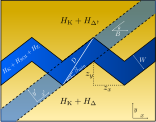
\includegraphics[width=0.75\columnwidth]{images/zigzag_methods.pdf}
		\caption{Schematic of the system, along with relevant dimensions, and the quasiclassical approach.
		The $x^\prime, y^\prime$ axis depicts the rotated frame for the quasiclassical estimate.
		The white trajectory indicates the estimate taken for the longest trajectory allowed by a zigzag.
		\label{fig:zigzag_methods}}
		\end{figure}

		\comment{We make an analogy between the cutoff of long trajectories to the cutoff of high momenta.}
		We hypothesize that the increase of the topological gap in a zigzag is due to the cutoff of modes on the Fermi surface with long trajectories.
		In order to substantiate that this is indeed the driving mechanism behind the improvement, we propose an analogy using the bandstructure of a regular SNS junction.

		\comment{We map the zigzag to an infinite SNS junction with tilted magnetic field and a range of forbidden momenta.}
		We take a single diagonal section of a zigzag, and map it to a normal, infinite SNS junction.
		We assume that the zigzag is shaped such that there is no straight trajectory possible through the system anymore.
		The system is depicted in Fig.~\ref{fig:zigzag_methods}, along with the set of axes with $x^\prime$ and $y^\prime$.
		Note that the magnetic field has an angle $\theta$ with respect to the $x^\prime$ axis.
		We identify trajectories cut off by the zigzag with a particular range of forbidden momenta.
		By then analysing the bandstructure of this infinite SNS junction, we can give an estimate the resulting gap of the device.
		As the system is only momentum localized in the $x$ direction (the translationally invariant direction), we only control $\kx$.
		Denoting the set of allowed momenta by $\Omega$, the equation for the estimated topological gap becomes,
		
		\begin{equation}
			\Delta_\text{topological} = \min_{\kx\in\Omega} \left| E(\kx) \right|
			\label{eq:definition_gap}
		\end{equation}
		
		\comment{We first link the long trajectories to a maximum allowed angle.}
		In the infinite system, the long trajectories have a small angle with respect to the $x^\prime$ axis.
		By defining a minimum angle, we thus can filter out the long trajectories.
		We define this angle $\beta_\text{min}$ by identifying it with the angle of the longest trajectory from one side of the superconductor to the other: see Fig.~\ref{fig:zigzag_methods}.
		Note that longer trajectories exist, by `grazing' the concave corners of the zigzag.
		We suspect that this `grazing' leads to physics which cannot be captured in this simple model, and we thus choose to restrict this method for systems where the chosen trajectory is indeed a good approximation of the longest path.

        We identify the momentum with its angle by defining it through the reciprocal of the component velocities, given by Eq.~\eqref{eq:methods_angle_of_state}. Note that $k_1$ and $k_2$ are the momenta as defined in Eq.~\eqref{eq:momenta_short_junction}.

        \begin{equation}
        \tan (\beta) = \left.\frac{v_y}{v_x}\right|_{E=E_F} = \left.\frac{ \frac{\de E}{\de k_y} }{ \frac{\de E}{\de k_x} } \right|_{E=E_F}=
        \begin{dcases}
        \frac{\hbar ^2 k_1}{\frac{\alpha  \meff \left(\alpha  k_x-\text{Ez} \sin (\theta )\right)}{\sqrt{\text{Ez}^2+\alpha  k_x \left(\alpha  k_x-2 \text{Ez} \sin (\theta )\right)}}+\hbar ^2 k_x} & \text{band 1}\\
        \frac{\hbar ^2 k_2}{\frac{\alpha  \meff \left(\text{Ez} \sin (\theta )-\alpha  k_x\right)}{\sqrt{\text{Ez}^2+\alpha  k_x \left(\alpha  k_x-2 \text{Ez} \sin (\theta )\right)}}+\hbar ^2 k_x} & \text{band 2}
        \end{dcases}
        \label{eq:methods_angle_of_state}
        \end{equation}
		
        We estimate the restriction of the domain for the momentum by geometrically calculating the minimum angle, as depicted in Fig.\ref{fig:zigzag_methods}. The result:

        \begin{align}
        	\tan \left(\beta_\text{min} \right) = \frac{W}{\sqrt{D^2 - W^2}} \label{eq:beta_min}\\
        	D = \sqrt{z_x^2 + \left(z_y + W \sqrt{1 + \left(\frac{z_y}{z_x}\right)^2}\right)^2} \nonumber
        \end{align}

        The condition for the restricted momentum becomes:
        \begin{equation}
        	\tan \left(\beta\right) \geq \tan \left(\beta_\text{min}\right)
        	\label{eq:restriction_momentum}
        \end{equation}